\chapter{Temo: Sumi du kubojn}
{ }\hfill\textbf{Nivelo:} Meza

Kiam oni ^jetas du kubojn kaj kalkulas la tuton de poentoj de amba^u
kuboj, oni akiras entjeron inter $2$ kaj $12$.  ^Ci tie, ni vidos la
distribuon de la diversaj rezultoj kaj ^gin reprezentos per malgranda
grafiko.

\section{Simuli ^jeti kubon}
Por simuli ^jeton de kubo, ni uzos la primitivon \texttt{hazardon}.  Jen kiel procedi.

\texttt{hazardon 6} $\longrightarrow$ redonas entjeron hazarde
elektitan el $0$, $1$, $2$, $3$, $4$, $5$.

Tial, \texttt{(hazardon 6) + 1} redonas entjeron elektitan el $1$,
$2$, $3$, $4$, $5$, $6$.  Rimarku ja la parentezojn; alie l'
interpretilo Logo komprenus \texttt{hazardon 7}.  Por ^spari l'
parentezojn, oni povas tajpi \texttt{1 + hazardon 6}.

Oni difinu tiel la proceduron \texttt{^jetu} kiu simulas ^jeti
ludkubon.
\begin{verbatim}
 por ĵetu
   sendu 1 + hazardon 6
 fino
\end{verbatim}
 \section{La programo}
 Ni uzos la moduson plur-testudan.  Por tiel havi plurajn testudojn
 sur l' ekran', oni uzu la primitivon \texttt{testudon\_provizu}
 sekvitan de la numero de la testudo kiun oni volas elekti.

 Bona skemo valoras pli ol mil klarigoj...
\begin{center}
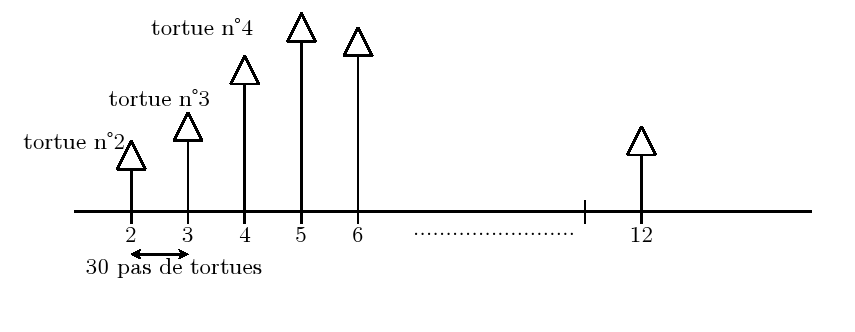
\includegraphics[scale=0.45]{bildoj/somme-des-schema.png}
\end{center}
\vspace{0.5cm} ^Ciu testudo numerata de $2$ ^gis $12$ anta^ueniros unu
testudpa^son kiam la sumo de la du kuboj ^jetitaj estas egala a ^gia
numero.  Por ekzemplo, se la kubo sumi^gas $8$, la testudo $8$a
anta^ueniru unu pa^son.  Inter ^ciuj du testudoj estu $30$
testudpa^soj horizontale.

Oni lokos la testudojn per koordinatoj.
\begin{itemize}
 \item  La testudo n\degre2 estu lokita en $(-150;0)$
 \item  La testudo n\degre3 estu lokita en $(-120;0)$
 \item  La testudo n\degre4 estu lokita en $(-90;0)$
 \item  La testudo n\degre5 estu lokita en $(-60;0)$\\
\begin{minipage}{8 cm}
\begin{center}
 $\vdots$
\end{center}
\end{minipage}
\end{itemize}
\begin{verbatim}
 testudon_provizu 2 sitp [-150 0]
 testudon_provizu 3 sitp [-120 0]
 testudon_provizu 4 sitp  [-90 0]
 testudon_provizu 5 sitp  [-60 0]
 testudon_provizu 6 sitp  [-30 0]
.....
\end{verbatim}
Pli bone ol tajpi $11$ fojojn preska^u la saman komandlinion, oni
a^utomatigu tion uzante la primitivon \texttt{ripetupor}.  Per tiu
primitivo, oni povas havigi al variablo sekvencon de valoroj prenitaj
en intervalo la^u samaj spacoj.  ^Ci tie, oni volas ke la variablo
\texttt{:i} prenu sinsekve la valorojn $2$, $3$, $4$... $12$.  Oni
tajpu:

\texttt{ripetu por [i 2 12] [ listo de rulotaj instrukcioj ]}

Por loki la testudojn, oni kreu do la proceduron \texttt{pretigu}
\begin{verbatim}
por pretigu
  ev tdk
  ripetupor [i 2 12]  
      [# Loku la testudon
       testudon_provizu :i sitp liston -150+(:i-2)*30 0
       # Skribu la numeron de la testudo apude sube
       l man 15 etikedu :i an 15 ml]
fino
\end{verbatim}

Bone komprenu la formulon \texttt{-150+(:i-2)*30}.  Oni ekiras de
$-150$; poste por ^ciu nova testudo oni aldonas $30$.  Provu per la
diversaj valoroj de \texttt{:i} se vi ne estas konvinkita.

Finfine jen la programo:
\begin{verbatim}
por ĵeti
 sendu 1 + hazardon 6
fino

por pretiu
  ev tdk
  ripetupor [i 2 12]  
      [# Loku la testudon
       testudon_provizu :i sitp liston -150+(:i-2)*30 0
       # Skribu la numeron de la testudo apude sube
       l man 15 etikedu :i an 15 ml]
fino

por startu
pretigu
# Realigu 1000 provoj
ripetu 1000 
  [provizu "sumo ĵetu+ĵetu
   testudon_provizu :sumo an 1]
# Skribu la frekvencojn de la ĵetado
ripetupor [i 2 12] 
 [testudon_provizu :i
  # L' ordinato de l' testudo reprezentas la nombron de ĵetoj
  loke_provizu "efika lastan sit 
  l an 10 mdn 90 an 10 dn 90 ml etikedu :efika/1000*100]
fino
\end{verbatim}

Jen ^generaligo de tiu programo.  Oni demandos al l' uzulo la nombron
de deziratajn kubojn kaj la nombron de ^jetojn farotajn.
\begin{verbatim}
por ĵetu
lokp "sumo 0
ripetu :kuboj 
  [lokp "sumo :sumo + 1 + hazardon 6]
sendu :sumo
fino

por pretigu
  ev tdk testudkiomon_provizu :maks+1
  ripetupor fr list "i :min :maks 
     [# Loku la testudon
      testudon_provizu :i sitp list (:min-:maks)/2*30+(:i-:min)*30 0
      # Skribu la numeron de la testudo apude sube
      l man 15 etikedu :i an 15 ml]
fino

por startu
leg [Nombro de kuboj:] "kuboj
se ne nombra? :kuboj [s [La nombro enigita ne estas valida!] haltu]
provizu "min :kuboj
provizu "maks 6*:kuboj
leg [Nombro de ĵetoj realigotaj] "ĵetoj
se ne nombra? :ĵetoj [s [La nombro enigita ne estas valida!] haltu]
pretigu
# Realigu 1000 provoj
ripetu :ĵetoj 
  [testudon_provizu ĵetu an 1]
# Ŝkribu la frekvencojn de la ĵetoj
ripetupor fr list "i :min :maks 
  [testudon_provizu :i
   # L' ordinato de l' testudo reprezentas la nombron de ĵetoj
   lokp "efika lastan sit 
   # Oni proksimumu je 0.1
   l an 10 mdn 90 an 10 dn 90 ml etikedu (entjeran :efika/:ĵetoj*1000) / 10]
fino

\end{verbatim}
